\paper{2015}

\question
\begin{parts}
    \part[5]
    Give a formal definition of a 
    deterministic finite-state automaton (DFA).
    \begin{solution}
        A \textbf{DFA} is a $5$-tuple $(Q, \Sigma, \delta, q_0, F)$
        where
        \begin{enumerate}
            \item $Q$ is a finite set of states;
            \item $\Sigma$ is a finite alphabet;
            \item $\delta: Q \times \Sigma \to Q$ 
                is a transition function;
            \item $q_0 \in Q$ is the initial state; and
            \item $F \subset Q$ is a set of accept states.
        \end{enumerate}
    \end{solution}

    \part[8]
    Tranform the non-deterministic finite-state automaton (NFA),
    whose transition function is given in the table below 
    where $A$ is the start state and $D$ is the only accept state,
    into a DFA.
    \begin{center}
        \begin{tabular}{ccccc}
            \toprule
                          & $A$   & $B$ & $C$ & $D$ \\
            \midrule
            $0$           & $A,B$ & $C$ &     &     \\
            $1$           & $A$   & $C$ & $D$ &     \\
            $\varepsilon$ &       &     &     & $D$ \\
            \bottomrule
        \end{tabular}
    \end{center}
    \begin{solution}
        Our transition table for our DFA is as follows. 
        \vspace{1em}
        \begin{center}
            \begin{tabular}{ccccccccc}
                \toprule
                & $A$ & $A,B$ & $A,B,C$ & $A,C,D$ & $A,C$ & $A,D$ & $D$ & $\varnothing$ \\
                \midrule
                $0$ & $A,B$ & $A,B,C$ & $A,B,C$ & $A,B$ & $A,B$ & $A,B$ & $\varnothing$ & $\varnothing$\\
                $1$ & $A$ & $A,C$ & $A,C,D$ & $A,D$ & $A,D$ & $A$ & $\varnothing$ & $\varnothing$ \\
                $\varepsilon$ & $\varnothing$ & $\varnothing$ & $\varnothing$ 
                              & $D$ & $\varnothing$ & $D$ 
                              & $D$ & $\varnothing$ \\
                \bottomrule
            \end{tabular}
        \end{center}
        \vspace{1em}
        Here our start state is $A$ and our accept states are all states with $D$
        in it, so $\{A,C,D\}$, $\{A,D\}$, and $\{D\}$.
    \end{solution}

    \part[7]
    Prove that the language
    \[
        \left\{
            a^{n^2} : n \in \N
        \right\}
    \]
    is not context-free.
    \begin{solution}
        \emph{
            I am not too sure whether or not context-free languages
            are covered this year, but it going to be assumed that
            we know that if a language is context-free, it is also
            regular.
        }
        Assume that the language above, $L$, is context-free.
        Therefore, it is regular.
        Let $p$ be the \emph{pumping length} of $L$, by the pumping lemma
        for all $w \in L$ with $\abs w \geq p$ we can express
        $w = xyz$ where $\abs y \geq 1$, $\abs{xy} \leq p$, and $xy^iz \in L$
        for all $i \geq 0$.
        Now let us consider the word $w = a^{p^2} = a^la^ma^{p^2 - l - m}$
        with $m \geq 1$ and $l \geq 0$.
        As $l + m \leq p$, $m \leq p$.
        Then
        \[
            p^2 + m \leq p^2 + p < p^2 + 2p + 1 = (p+1)^2;
        \]
        so, $p^2 < p^2 + m < (p+1)^2$.
        Therefore, $p^2 + m$ lies between two squares
        and so $a^{p^2+m} \not\in L$.
        $a^l \left( a^m \right)^2 a^{p^2 - l - m} \in L$
        by the pumping lemma, but $a^l \left( a^m \right)^2 a^{p^2 - l - m} = a^{p^2+m}$,
        a contradiction.
        Therefore, $L$ is not context-free.
    \end{solution}

    \part[5]
    Give an algorithm that decides whether 
    $L(M_1) \subset L(M_2)$
    for any two DFAs $M_1$ and $M_2$.
    (Here $L(M_i)$ denotes the language recognised by $M_i$.)
    \begin{solution}
        Let $\Sigma$ be the alphabet for a DFA.
        Then, for all $w \in \Sigma^\star$
        we will simulate $M_1$ on $w$:
        \begin{enumerate}
            \item if $M_1$ accepts, we continue;
            \item if $M_1$ rejects we go back to the start with the next $w$.
        \end{enumerate}
        Now, given that $M_1$ accepted, we simulate $M_2$ on $w$:
        \begin{enumerate}
            \item if $M_2$ accepts, we continue;
            \item if $M_2$ rejects, we reject.
        \end{enumerate}
        Now, given that $M_2$ also accepted, we restart with the next $w$.
        If there are no more $w$ and we have not rejected yet, we accept.
    \end{solution}
\end{parts}

\question
\begin{parts}
    \part[6]
    Give a formal definition of a 
    non-determinstic finite-state automaton (NFA).
    \begin{solution}
        A \textbf{NFA} is a $5$-tuple $(Q, \Sigma, \delta, q_0, F)$
        where
        \begin{enumerate}
            \item $Q$ is a finite set of states;
            \item $\Sigma$ is a finite alphabet;
            \item $\delta: Q \times \Sigma \to \mathcal P(Q)$
                is a transition function;
            \item $q_0 \in Q$ is an initial state; and
            \item $F \subset Q$ is a set of accept states.
        \end{enumerate}
    \end{solution}

    \part[8]
    Minimise the DFA whose transition function 
    is given in the table below,
    \begin{center}
        \begin{tabular}{cccccccccc}
            \toprule
                & $A$ & $B$ & $C$ & $D$ & $E$ & $F$ & $G$ & $H$ & $I$ \\
            \midrule
            $a$ & $B$ & $E$ & $E$ & $A$ & $I$ & $D$ & $B$ & $D$ & $B$ \\
            $b$ & $D$ & $F$ & $G$ & $B$ & $H$ & $I$ & $I$ & $E$ & $F$ \\
            \bottomrule
        \end{tabular}
    \end{center}
    where $A$ is the start state, and $D$ and $G$ are the accepting states.
    \begin{solution}
        We will implement the \emph{team-splitting algorithm}
        (though I don't think this is the name in the literature).
        First we \emph{disqualify} $C$ and $G$.
        Now we partition our states as so:
        \[
            \{A,B,E,F,H,I\}, \{D\}.
        \]
        Now we split the first set on a $a$-ball:
        \[
            \{A,B,E,I\}, \{F,H\}, \{D\}.
        \]
        Split the first set on a $b$-ball:
        \[
            \{A\}, \{B,E,I\}, \{F,H\}, \{D\}.
        \]
        Now all teams agree; hence we have minimised our DFA.
        We get the following transition function
        \begin{center}
            \begin{tabular}{ccccc}
                \toprule
                    & $A$ & $B$ & $C$ & $D$ \\
                \midrule
                $a$ & $B$ & $B$ & $D$ & $A$ \\
                $b$ & $D$ & $C$ & $B$ & $B$ \\
                \bottomrule
            \end{tabular}
        \end{center}
        where $A$ is our start sate and $D$ is the sole accept state.
    \end{solution}

    \part[7]
    Explain how a correctly formed arithmetic expression over variables
    $a$, $b$, and $c$
    that contains additions, multiplications, and brackets
    can be recognised by a DFA with a counter.
    (Such a DFA can increment and decrement the counter on each
    transition as well as test it for zero.)
    \begin{solution}
        % todo
    \end{solution}

    \part[4]
    Is it algorithmically decidable whether a Turing-decidable
    language is finite?
    Justify your answer.
    \begin{solution}
        By Rice's theorem,
        any property of languages recognised by Turing machines
        is undecidable;
        therefore, it is undeciable whether a Turing-decidable language
        is finite.
    \end{solution}
\end{parts}

\question
\begin{parts}
    \part[7]
    Give a formal definition of a push-down automaton (PDA).
    \begin{solution}
        A \textbf{push-down automaton} is a $7$-tuple
        \[
            M = (Q, \Sigma, \Pi, \delta, q_0, Z, F)
        \]
        where
        \begin{enumerate}
            \item $Q$ is a finite set of states;
            \item $\Sigma$ is a finite set called the input alphabet;
            \item $\Gamma$ is a finite set called the stack alphabet;
            \item $\delta: Q \times (\Sigma \cup \{\varepsilon\}) \times \Gamma \times Q \times \Gamma^\star$
                called the transition relation;
            \item $q_0 \in Q$ is the start state;
            \item $Z \in \Gamma$ is the initial stack symbol; and
            \item $F \subset Q$ is the set of accepting states.
        \end{enumerate}
    \end{solution}

    \part[6]
    Convert into a regular expression the DFA whose transition function
    is given in the table below,
    \begin{center}
        \begin{tabular}{cccc}
            \toprule
              & $A$ & $B$ & $C$ \\
            \midrule
            0 & $B$ & $C$ & $B$ \\
            1 & $B$ & $B$ & $C$ \\
            \bottomrule
        \end{tabular}
    \end{center}
    where $A$ is the start state, and $B$ is the only accepting state.
    \begin{solution}
        \begin{center}
            \ttfamily
            (0|1)((01*0)|1)*.
        \end{center}
    \end{solution}

    \part[6]
    Show that the language
    \[
        \{
            0^ku\#v : u,v \in \{a,b\}^\star :
            \text{$u$ and $v$ have a common subword of length $k \in \N$}
        \}
    \]
    is context-free.
    % todo now on

    \part[6]
    Give an algorithm that decides whether a word can be generated by
    a context-sensitive grammar.
\end{parts}

\question
\begin{parts}
    \part[5]
    Give a formal definition of a context-free grammar (CFG).

    \part[7]
    Prove that the language
    \[
        \{
            w \in \{0,1\}^\star :
            \text{if the length of $w$ is odd, then the middle symbol is $0$}
        \}
    \]
    is not regular.
    \begin{solution}
        Assume that the language above, $L$, is regular.
        Then consider the string $w = 1^p01^p \in L$ where $p$
        is the pumping length.
        By the pumping lemma, 
        we have that $w = xyz$
        for some strings $x$, $y$, and $z$
        where
        \begin{enumerate}
            \item $\abs x \geq$;
            \item $\abs{xy} \leq p$; and
            \item $xy^iz \in L$ for all $i \geq 0$.
        \end{enumerate}
        So $x = 1^i$, $y = 1^j$, and $z = 1^{p-i-j}01^p$
        for some $i$ and $j$ where $i \geq 0$ and $j \geq 1$.
        Now
        \[
            xy^3z = 1^i1^{3j}1^{p-i-j}01^p = 1^{p+2j}01^p.
        \]
        As $\abs{xy^3z} = p+2j+1+p = 2(p+j)+1$, it has odd length;
        but the middle character is 1 as $j \neq 0$.
        Therefore: $xy^3z \not\in L$, a contradiction.
        Therefore $L$ is not regular.
    \end{solution}

    \part[7]
    Design a DFA that recognises precisely the words that contain the string
    \emph{``abbabab''}
    as a subword.
    \begin{solution}
        \begin{center}
            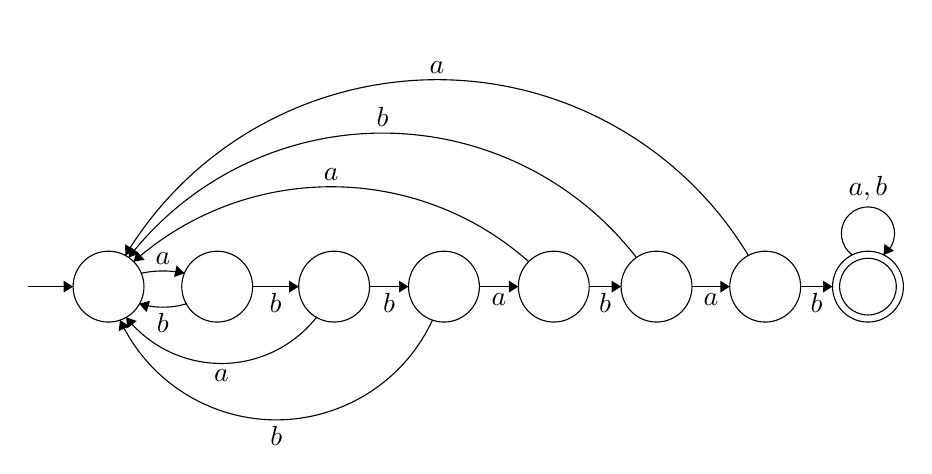
\begin{tikzpicture}[scale=0.15]
                \tikzstyle{every node}+=[inner sep=0pt]
                \draw [black] (8.3,-26.5) circle (3);
                \draw [black] (17.5,-26.5) circle (3);
                \draw [black] (27.4,-26.5) circle (3);
                \draw [black] (36.7,-26.5) circle (3);
                \draw [black] (46,-26.5) circle (3);
                \draw [black] (54.7,-26.5) circle (3);
                \draw [black] (63.9,-26.5) circle (3);
                \draw [black] (72.6,-26.5) circle (3);
                \draw [black] (72.6,-26.5) circle (2.4);
                \draw [black] (11.063,-25.369) arc (102.29553:77.70447:8.628);
                \fill [black] (14.74,-25.37) -- (14.06,-24.71) -- (13.85,-25.69);
                \draw (12.9,-24.67) node [above] {$a$};
                \draw [black] (1.5,-26.5) -- (5.3,-26.5);
                \fill [black] (5.3,-26.5) -- (4.5,-26) -- (4.5,-27);
                \draw [black] (20.5,-26.5) -- (24.4,-26.5);
                \fill [black] (24.4,-26.5) -- (23.6,-26) -- (23.6,-27);
                \draw (22.45,-27) node [below] {$b$};
                \draw [black] (30.4,-26.5) -- (33.7,-26.5);
                \fill [black] (33.7,-26.5) -- (32.9,-26) -- (32.9,-27);
                \draw (32.05,-27) node [below] {$b$};
                \draw [black] (39.7,-26.5) -- (43,-26.5);
                \fill [black] (43,-26.5) -- (42.2,-26) -- (42.2,-27);
                \draw (41.35,-27) node [below] {$a$};
                \draw [black] (49,-26.5) -- (51.7,-26.5);
                \fill [black] (51.7,-26.5) -- (50.9,-26) -- (50.9,-27);
                \draw (50.35,-27) node [below] {$b$};
                \draw [black] (57.7,-26.5) -- (60.9,-26.5);
                \fill [black] (60.9,-26.5) -- (60.1,-26) -- (60.1,-27);
                \draw (59.3,-27) node [below] {$a$};
                \draw [black] (66.9,-26.5) -- (69.6,-26.5);
                \fill [black] (69.6,-26.5) -- (68.8,-26) -- (68.8,-27);
                \draw (68.25,-27) node [below] {$b$};
                \draw [black] (71.277,-23.82) arc (234:-54:2.25);
                \draw (72.6,-19.25) node [above] {$a,b$};
                \fill [black] (73.92,-23.82) -- (74.8,-23.47) -- (73.99,-22.88);
                \draw [black] (14.899,-27.948) arc (-73.26181:-106.73819:6.943);
                \fill [black] (10.9,-27.95) -- (11.52,-28.66) -- (11.81,-27.7);
                \draw (12.9,-28.74) node [below] {$b$};
                \draw [black] (25.913,-29.093) arc (-38.21372:-141.78628:10.262);
                \fill [black] (9.79,-29.09) -- (9.89,-30.03) -- (10.68,-29.41);
                \draw (17.85,-33.51) node [below] {$a$};
                \draw [black] (35.726,-29.332) arc (-24.87353:-155.12647:14.578);
                \fill [black] (9.27,-29.33) -- (9.16,-30.27) -- (10.06,-29.85);
                \draw (22.5,-38.28) node [below] {$b$};
                \draw [black] (10.423,-24.383) arc (131.52004:48.47996:25.234);
                \fill [black] (10.42,-24.38) -- (11.35,-24.23) -- (10.69,-23.48);
                \draw (27.15,-17.54) node [above] {$a$};
                \draw [black] (10.004,-24.033) arc (142.21463:37.78537:27.2);
                \fill [black] (10,-24.03) -- (10.89,-23.71) -- (10.1,-23.09);
                \draw (31.5,-13) node [above] {$b$};
                \draw [black] (9.724,-23.861) arc (148.85845:31.14155:30.817);
                \fill [black] (9.72,-23.86) -- (10.57,-23.43) -- (9.71,-22.92);
                \draw (36.1,-8.48) node [above] {$a$};
            \end{tikzpicture}
        \end{center} 
    \end{solution}

    \part[6]
    Show that the language
    \[
        \{
            uv : u,v \in \{0,1\}^\star: \abs u = \abs v, u \neq v
        \}
    \]
    is context-free.
    \begin{solution}
        \emph{
            This looks harder then just showing that the language is not regular,
            and context-free languages have not been covered this year.
        }
    \end{solution}
\end{parts}
